\documentclass[x11names,dvipsnames,table,aspectratio=169]{beamer}
\usepackage{beamerthemesplit}
\usepackage{wrapfig}
\usetheme{SPbGU}
\usepackage{pdfpages}
\usepackage{amsmath}
\usepackage{cmap} 
\usepackage[T2A]{fontenc} 
\usepackage[utf8]{inputenc}
\usepackage[english,russian]{babel}
\usepackage{indentfirst}
\usepackage{amsmath}
\usepackage{tikz}
\usepackage{multirow}
\usepackage[noend]{algpseudocode}
\usepackage{algorithm}
\usepackage{algorithmicx}
\usetikzlibrary{shapes,arrows}
\usepackage{fancyvrb}
\usepackage{colortbl}
\usepackage{appendixnumberbeamer}

\usetikzlibrary{automata, arrows.meta, positioning}
\usetikzlibrary{decorations.pathreplacing}

\beamertemplatenavigationsymbolsempty


\title[]{Экспериментальное исследование алгоритмов контекстно-свободной достижимости применительно к задачам статического анализа кода}
\institute[СПбГУ]{
Санкт-Петербургский государственный университет \\
Кафедра системного программирования }

\author[Владимир Кутуев]{Кутуев Владимир Александрович,  \\
  \and  
    {\bfseries Научный руководитель:} к.\,ф.-м.\,н., доцент Григорьев С.\,В. \\ 
    {\bfseries Рецензент:} старший преподаватель СПбПУ, Беляев М.\,А. \\ 
}

\date{6 июня 2023г.}

\begin{document}
{
\begin{frame}
    \begin{center}
        
\includegraphics[width=1.7cm]{pictures/SPbGU_Logo.png}
    \end{center}
    \titlepage
\end{frame}
}

\begin{frame}[fragile]
  \transwipe[direction=90]
  \frametitle{КС-достижимость}
  \begin{itemize}
    \item Область применения
    \begin{itemize}
        \item Анализ RDF данных
        \item Биониформатика
        \item Статический анализ кода
    \end{itemize}
    \item Алгоритмы
    \begin{itemize}
        \item Основанные на алгоритмах синтаксического анализа
        \begin{itemize}
            \item LL
            \item GLL
            \item SYK
            \item ...
        \end{itemize}
        \item Основанные на операциях линейной алгебры
        \begin{itemize}
            \item Алгоритм, основанный на умножении матриц
            \item Алгоритм, основанный на произведении Кронекера
        \end{itemize}
    \end{itemize}
  \end{itemize}
  
\end{frame}

            
\begin{frame}
  \transwipe[direction=90]
  \frametitle{Постановка задачи}
  
  \textbf{Цель} работы --- экспериментально исследовать алгоритмы КС-достижимости в задаче статического анализа кода

  \textbf{Задачи}:
  \begin{itemize}
    \item Оптимизировать реализации алгоритмов, основанных на операциях линейной алгебры
    \item Рассмотреть возможность применения алгоритмов, основанных на операциях линейной алгебры, для Points-to анализа, учитывающего поля, и предложить модификацию алгоритма, подходящую для этого анализа
    \item Провести замеры производительности алгоритмов, основанных на операциях линейной алгебры, на графах, полученных по реальным программам, сравнить их с другими алгоритмами КС-достижимости
  \end{itemize}
\end{frame}


\begin{frame}
  \transwipe[direction=90]
  \frametitle{Данные для экспериментов}
  \begin{itemize}
    \item Для экспериментов были взяты графы из набора CFPQ\_Data\footnote{\url{https://github.com/FormalLanguageConstrainedPathQuerying/CFPQ_Data}}
    \item Анализ псевдонимов
    \begin{itemize}
        \item 5 небольших графов (число вершин --- до нескольких тысяч)
        \item 15 больших графов (число вершин --- несколько миллионов)
    \end{itemize}
    \item Points-to анализ, учитывающий поля
    \begin{itemize}
        \item 10 средних графов (число вершин --- десятки тысяч)
        \item 4 больших графа (число вершин --- сотни тысяч)
    \end{itemize}
  \end{itemize}
\end{frame}


\begin{frame}
  \transwipe[direction=90]
  \frametitle{Оптимизация реализации матричного алгоритма}
  \begin{itemize}
    \item Реализация матричного алгоритма CFPQ\_PyAlgo\footnote{\url{https://github.com/FormalLanguageConstrainedPathQuerying/CFPQ_PyAlgo}}
    \item BOOL.LOR\_LAND
    \begin{itemize}
        \item сложение --- LOR (дизъюнкция)
        \item умножение --- LAND (конъюнкция)
    \end{itemize}
    \item BOOL.ANY\_PAIR
    \begin{itemize}
        \item сложение --- ANY (выбирает любой из переданных аргументов)
        \item умножение --- PAIR (возвращает 1, если оба операнда --- присутствующие в матрице элементы)
    \end{itemize}
  \end{itemize}
  
  \begin{center}    
    \resizebox{.7\textwidth}{!}{
    \rowcolors{2}{black!2}{black!10}
    \begin{tabular}{|l|r|r|c|c|r|}
        \hline
        Граф & $|V|$ & $|E|$ & LOR\_LAND (сек.) & ANY\_PAIR (сек.) & Ускорение \\ \hline \hline
        wc & 332 & 269 & 0,006 & 0,006 & 1,00 \\
        bzip2 & 632 & 556 & 0,022 & 0,022 & 1,00 \\
        pr & 815 & 692 & 0,013 & 0,012 & 1,08 \\
        ls & 1 687 & 1 453 & 0,051 & 0,045 & 1,13 \\
        gzip & 2 687 & 2 293 & 0,038 & 0,030 & 1,26 \\
        apache & 1 721 418 & 1 510 411 & 683,58 & 536,70 & 1,27 \\ 
        init & 2 446 224 & 2 112 809 & 59,33 & 45,84 & 1,29 \\ \hline
    \end{tabular}%
   }
   \end{center}
\end{frame}


\begin{frame}
  \transwipe[direction=90]
  \frametitle{Алгоритмы, основанные на операциях линейной алгебры}
  \begin{itemize}
    \item Матричный алгоритм
    \begin{itemize}
        \item Основан на умножении булевых матриц
        \item Требует перевода грамматики в ослабленную нормальную форму Хомского, что значительно увеличивает её размер
        \item Производительность зависит от размера грамматики
    \end{itemize}
    \item Тензорный алгоритм
    \begin{itemize}
        \item Основан на произведении Кронекера булевых матриц
        \item КС-язык задаётся рекурсивным автоматом
        \item Рекурсивный автомат и граф представляются как композиция булевых матриц смежности для каждой метки на ребре
    \end{itemize}
  \end{itemize}

\end{frame}


\begin{frame}
  \transwipe[direction=90]
  \frametitle{Рекурсивный автомат}

\begin{itemize}
    \item Анализ псевдонимов
    
    \begin{tabular}{|c|c|}
    \hline
    MA & VA \\      
      \begin{minipage}{.35\textwidth}
      \scalebox{0.6}{
      \begin{tikzpicture}[node distance=1.0cm, auto] 
          \node (q0) [state, initial, initial text = {}] {$q_0$};
          \node (q1) [state, right = of q0] {$q_1$};
          \node (q2) [state, right = of q1] {$q_2$};
          \node (q3) [state, accepting, right = of q2] {$q_3$};
          
          \path [-stealth, thick]
              (q0) edge node[above] {$\overline{d}$} (q1)
              (q1) edge node[above] {$VA$} (q2)
              (q2) edge node[above] {$d$} (q3)
              ;
      \end{tikzpicture}
      }
      \end{minipage}
  
      &
      \begin{minipage}{.25\textwidth}
      \scalebox{0.6}{
      \begin{tikzpicture}[auto] 
          \node (q0) [state, accepting, initial, initial text = {}] {$q_4$};
          \node (q1) [state, accepting, right=2.7cm of q0] {$q_5$};
          \node (q2) [state, accepting, below=0.4cm of q0] {$q_6$};
          \node (q3) [state, accepting, below=0.4cm of q1] {$q_7$};
          
          \path [-stealth, thick]
              (q0) edge node[above] {$a$} (q1)
              (q0) edge [loop above] node[right] {$\overline{a}$}()
              (q0) edge[bend right] node[left] {$MA$} (q2)

              (q1) edge[loop above] node[right] {$a$}()
              (q1) edge[bend right] node[left] {$MA$} (q3)

              (q2) edge[bend right] node[right] {$\overline{a}$} (q0)
              (q2) edge node[below] {$a$} (q1)
              
              (q3) edge[bend right] node[right] {$a$} (q1)
              ;
      \end{tikzpicture} 
      }
      \end{minipage}
      \\
      & \\
      \hline
  
  \end{tabular}
% Points-to
\item Points-to анализ, учитывающий поля

  \begin{tabular}{|c|c|c|}
  \hline
  PointsTo & FlowsTo & Alias \\
    \begin{minipage}{.3\textwidth}
    \scalebox{0.6}{
    \begin{tikzpicture}[node distance=0.6cm, auto] 
        \node (q0) [state, initial, initial text = {}] {$q_0$};
        \node (q1) [state, accepting, below = of q0] {$q_1$};
        
        \node (q4) [right=1.7cm of q0] {$...$};
        
        \node (q2) [state, above=0.5cm of q4] {};
        \node (q3) [state, right=1.7cm of q2] {};
        
        \node (q5) [state, below=1.0cm of q4] {};
        \node (q6) [state, right=1.7cm of q5] {};
        
        \path [-stealth, thick]
            (q0) edge [loop above]  node[above left] {$assign$}()
            (q0) edge node[left] {$alloc$} (q1)
            
            (q0) edge[bend left] node[below right] {$load_{f_1}$} (q2)
            (q2) edge node[above] {$Alias$} (q3)
            (q3) edge node[below right] {$store_{f_1}$} (q0)
            
            (q0) edge[bend right] node[above right] {$load_{f_n}$} (q5)
            (q5) edge node[above] {$Alias$} (q6)
            (q6) edge node[above right] {$store_{f_n}$} (q0)
            ;
    \end{tikzpicture}
    }
    \end{minipage}

    &
\begin{minipage}{.3\textwidth}
\scalebox{0.6}{
    \begin{tikzpicture}[node distance=0.6cm] 
        \node (q0) [state, initial, initial text = {}] {$q_2$};
        \node (q1) [state, accepting, below = of q0] {$q_3$};
        
        \node (q4) [right=1.7cm of q1] {$...$};
        
        \node (q2) [state, above=1.0cm of q4] {};
        \node (q3) [state, right=1.7cm of q2] {};
        
        \node (q5) [state, below=0.5cm of q4] {};
        \node (q6) [state, right=1.7cm of q5] {};
        
        \path [-stealth, thick]
            (q0) edge node[left] {$\overline{alloc}$} (q1)
            (q1) edge [loop below] node[below left] {$\overline{assign}$}()
            
            (q1) edge[bend left] node[below right] {$\overline{store_{f_1}}$} (q2)
            (q2) edge node[above] {$Alias$} (q3)
            (q3) edge node[below right] {$\overline{load_{f_1}}$} (q1)
            
            (q1) edge[bend right] node[below] {$\overline{store_{f_n}}$} (q5)
            (q5) edge node[below] {$Alias$} (q6)
            (q6) edge node[above right] {$\overline{load_{f_n}}$} (q1);
    \end{tikzpicture} 
    }
    \end{minipage}
    &
\begin{minipage}{.12\textwidth}
\scalebox{0.6}{
    \begin{tikzpicture}[node distance=0.4cm] 
        \node (q0) [state, initial, initial text = {}] {$q_4$};
        \node (q1) [state, below = of q0] {$q_5$};
        \node (q2) [state, accepting, below = of q1] {$q_6$};
        \path [-stealth, thick]
            (q0) edge node[right] {$PointsTo$} (q1)
            (q1) edge node[right] {$FlowsTo$} (q2)
            ;
    \end{tikzpicture} 
    }
    \end{minipage}
    \\
    & & \\
    \hline

\end{tabular}
\end{itemize}
\end{frame}


\begin{frame}
  \transwipe[direction=90]
  \frametitle{Адаптация графа}
  \begin{tabular}{ccc}
  Исходные рёбра & Новая переменная & Результат \\
 
  \begin{tikzpicture}[node distance=2.0cm] 
        \node[] (1) {$x$};
        \node[] (2) [right of=1] {$y$};
        
        \draw[->] (1) to [out=45, in=135, looseness=1] node[midway, above] {$...$} (2);
        \draw[->] (1) to node[midway, below, sloped] {$assign$} (2); 
  \end{tikzpicture} 
  &
  z = y; x = z;
  & 
  \begin{tikzpicture}[node distance=2.0cm] 
        \node[] (1) {$x$};
        \node[] (2) [right of=1] {$z$};
        \node[] (3) [right of=2] {$y$};
        
        \draw[->] (1) -- node[midway, above, sloped] {$assign$} (2); 
        \draw[->] (2) -- node[midway, above, sloped] {$assign$} (3); 
        \draw[->] (1) to [out=45, in=135, looseness=1] node[midway, above] {$...$} (3);
  \end{tikzpicture} 
  \\
  \begin{tikzpicture}[node distance=2.0cm] 
        \node[] (1) {$x$};
        \node[] (2) [right of=1] {$y$};
        
        \draw[->] (1) to [out=45, in=135, looseness=1] node[midway, above] {$...$} (2);
        \draw[->] (1) to node[midway, below, sloped] {$store_f$} (2); 
  \end{tikzpicture} 
  &
  z = y; x.f = z;
  & 
  \begin{tikzpicture}[node distance=2.0cm] 
        \node[] (1) {$x$};
        \node[] (2) [right of=1] {$z$};
        \node[] (3) [right of=2] {$y$};
        
        \draw[->] (1) -- node[midway, above, sloped] {$store_f$} (2); 
        \draw[->] (2) -- node[midway, above, sloped] {$assign$} (3); 
        \draw[->] (1) to [out=45, in=135, looseness=1] node[midway, above] {$...$} (3);
  \end{tikzpicture} 
  \\
  \begin{tikzpicture}[node distance=2.0cm] 
        \node[] (1) {$x$};
        \node[] (2) [right of=1] {$y$};
        
        \draw[->] (1) to [out=45, in=135, looseness=1] node[midway, above] {$...$} (2);
        \draw[->] (1) to node[midway, below, sloped] {$load_f$} (2); 
  \end{tikzpicture} 
  &
  z = y.f; x = z;
  & 
  \begin{tikzpicture}[node distance=2.0cm] 
        \node[] (1) {$x$};
        \node[] (2) [right of=1] {$z$};
        \node[] (3) [right of=2] {$y$};
        
        \draw[->] (1) -- node[midway, above, sloped] {$assign$} (2); 
        \draw[->] (2) -- node[midway, above, sloped] {$load_f$} (3); 
        \draw[->] (1) to [out=45, in=135, looseness=1] node[midway, above] {$...$} (3);
  \end{tikzpicture} 
  \end{tabular}
\end{frame}


\begin{frame}
  \transwipe[direction=90]
  \frametitle{Представление с одним терминалом}
  \begin{itemize}
    \item Граф и рекурсивный автомат представляются матрицами смежности с целочисленными элементами
    \item Старшие биты содержат маску нетерминалов, младшие --- номер терминала \\
  \end{itemize}
  \centering {
    \scalebox{0.7}{
      \begin{tikzpicture}
        [
            box/.style={rectangle,draw=black, ultra thick, minimum size=1cm},
        ]
        \foreach \x in {0,1,2,3,4,5,6,7,8}
            \node[box] at (\x,0){};
        \draw[decorate,decoration={brace, amplitude=0.2cm,mirror},thick] (-.5,-.7) -- node[below=0.2cm]{Нетерминалы} (2.49,-.7);
        \draw[decorate,decoration={brace, amplitude=0.2cm, mirror},thick] (2.51,-.7) -- node[below=0.2cm]{Терминал} (8.5,-.7);
      \end{tikzpicture}
    }
  }
  \begin{itemize}
    \item Операция умножения элементов для произведения Кронекера
    \begin{itemize}
        \item $times(x, y) = (x_{nonterms} \& y_{nonterms} \neq 0 \ or\ x_{term} = y_{term} \neq 0)$
        \item В матрице-результате много элементов будет $false$
        \begin{itemize}
            \item Вычисление транзитивного замыкания потребует больше времени
            \item Нужно больше памяти под его хранение
        \end{itemize}
        \item Необходима фильтрация результата произведения Кронекера
    \end{itemize}
  \end{itemize}
\end{frame}


\begin{frame}
  \transwipe[direction=90]
  \frametitle{Фильтрация результатов}
  \begin{itemize}
      \item Реализация произведения Кронекера из библиотеки SuiteSparse:GraphBLAS\footnote{\url{https://github.com/DrTimothyAldenDavis/GraphBLAS}}
      \item Адаптированная реализация\footnote{\url{https://github.com/vkutuev/GraphBLAS/tree/vkutuev/kron}}, не выделяющая память под значения $false$
  \end{itemize}
  \begin{tabular}{cc}
      \begin{minipage}{.48\textwidth}
      \begin{figure}
        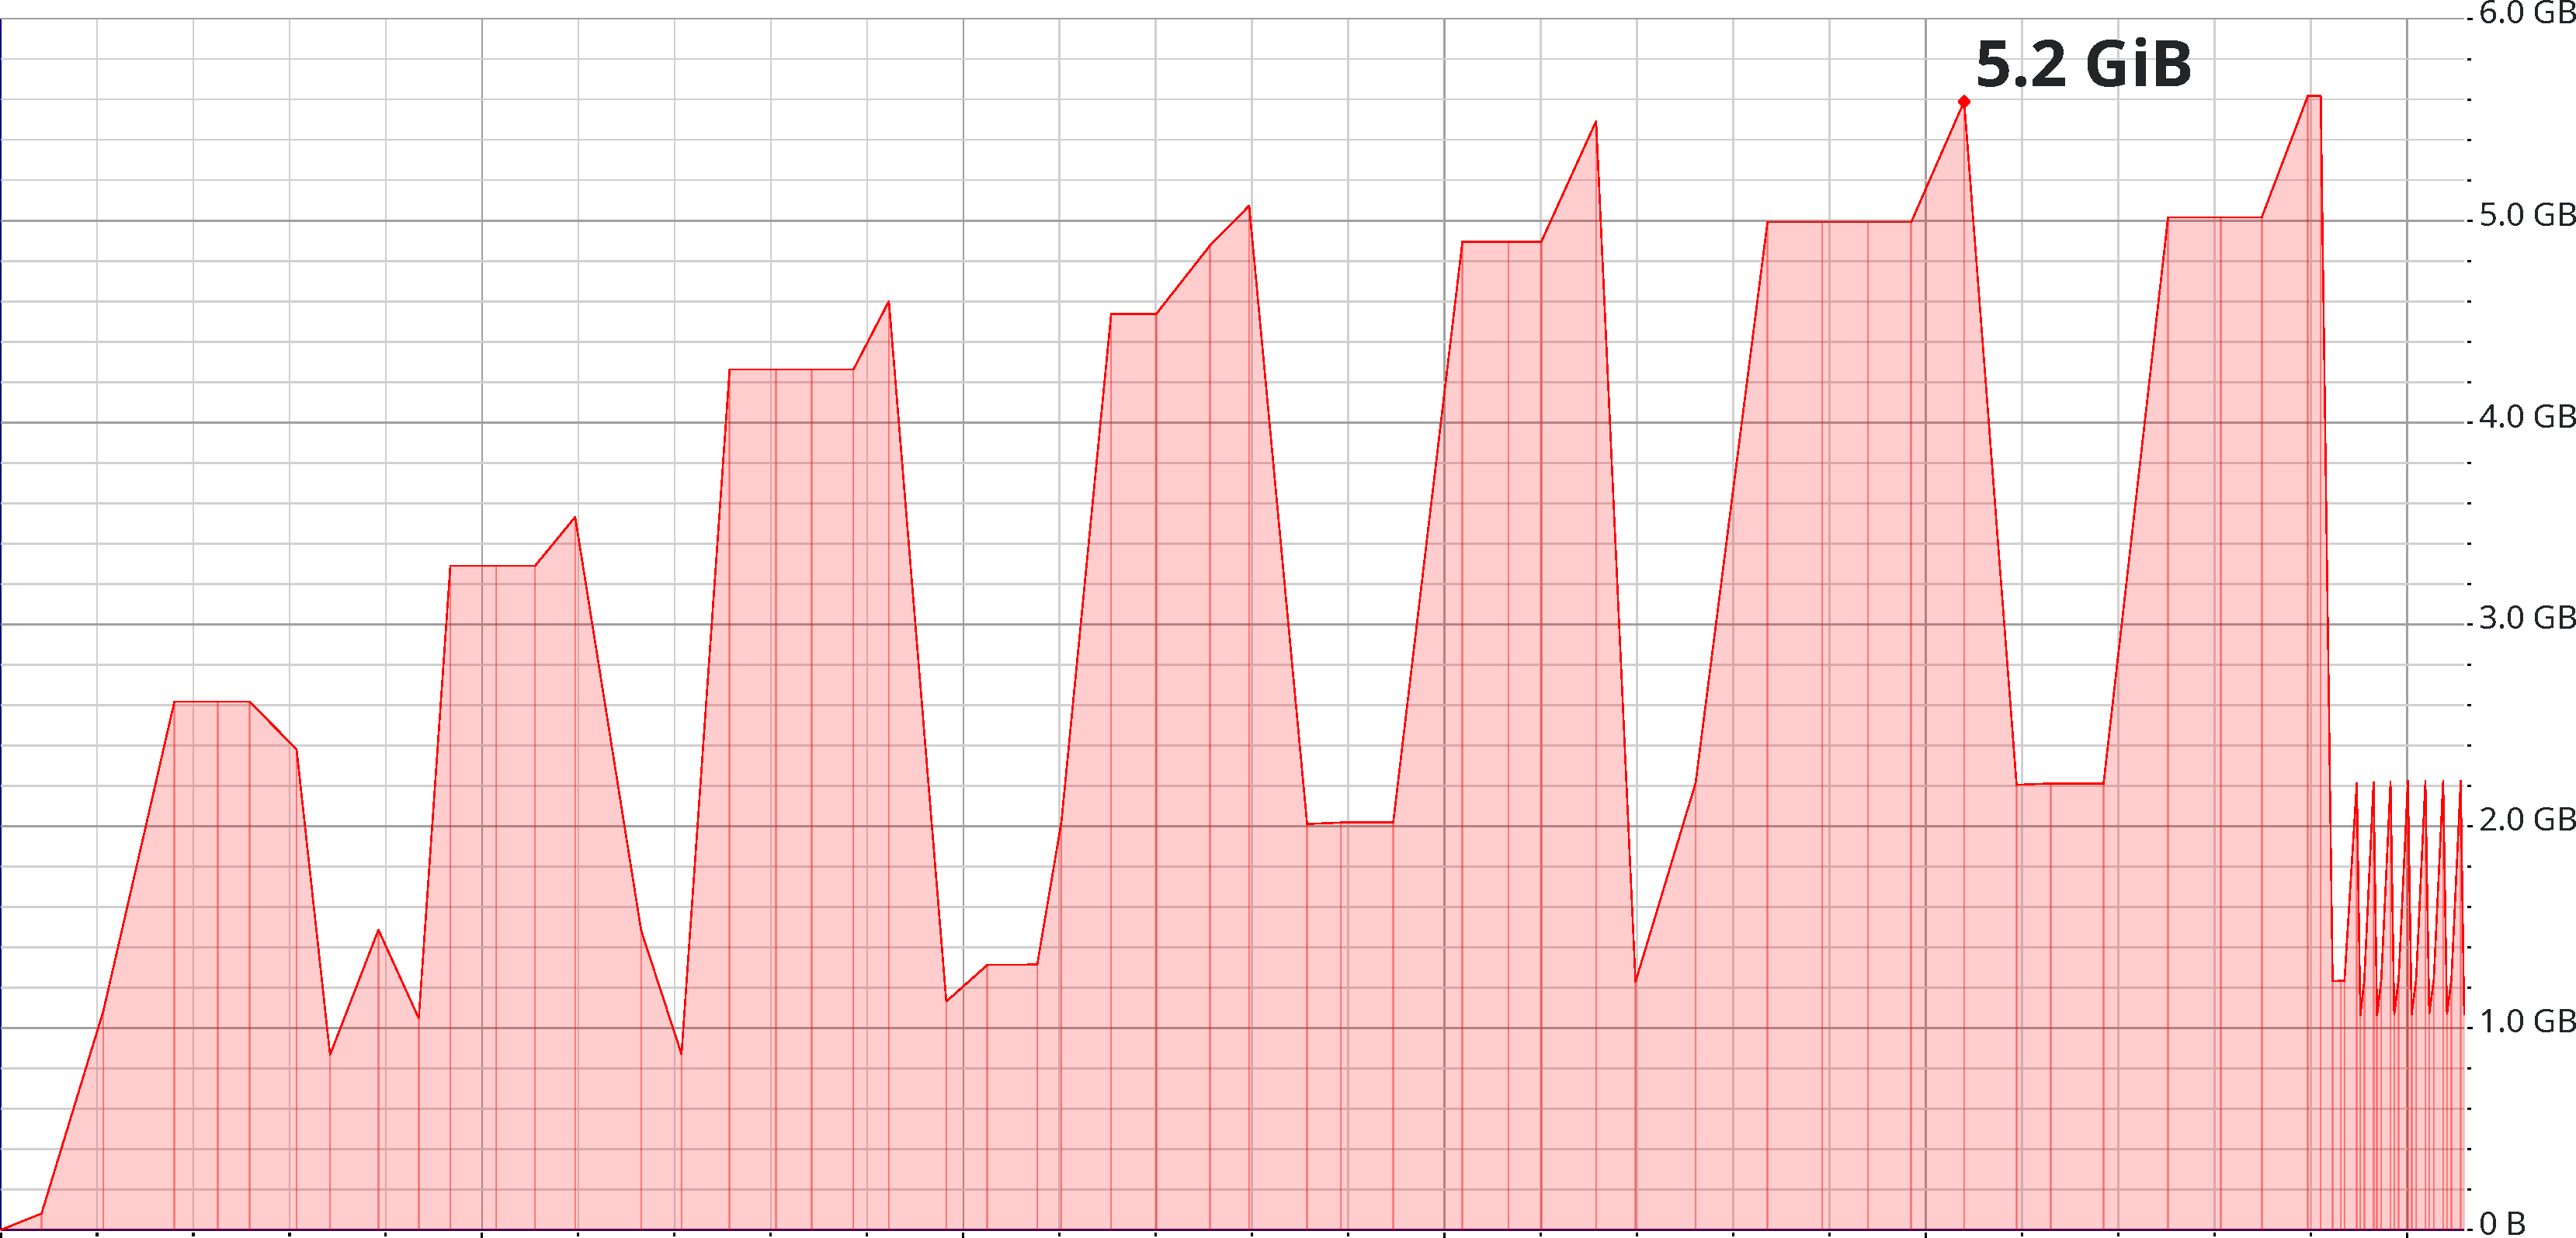
\includegraphics[width=\textwidth]{pictures/mem_prof_base.pdf}
        \caption{Стандартная реализация}
      \end{figure}
      \end{minipage}
      &
      \begin{minipage}{.48\textwidth}
      \begin{figure}
        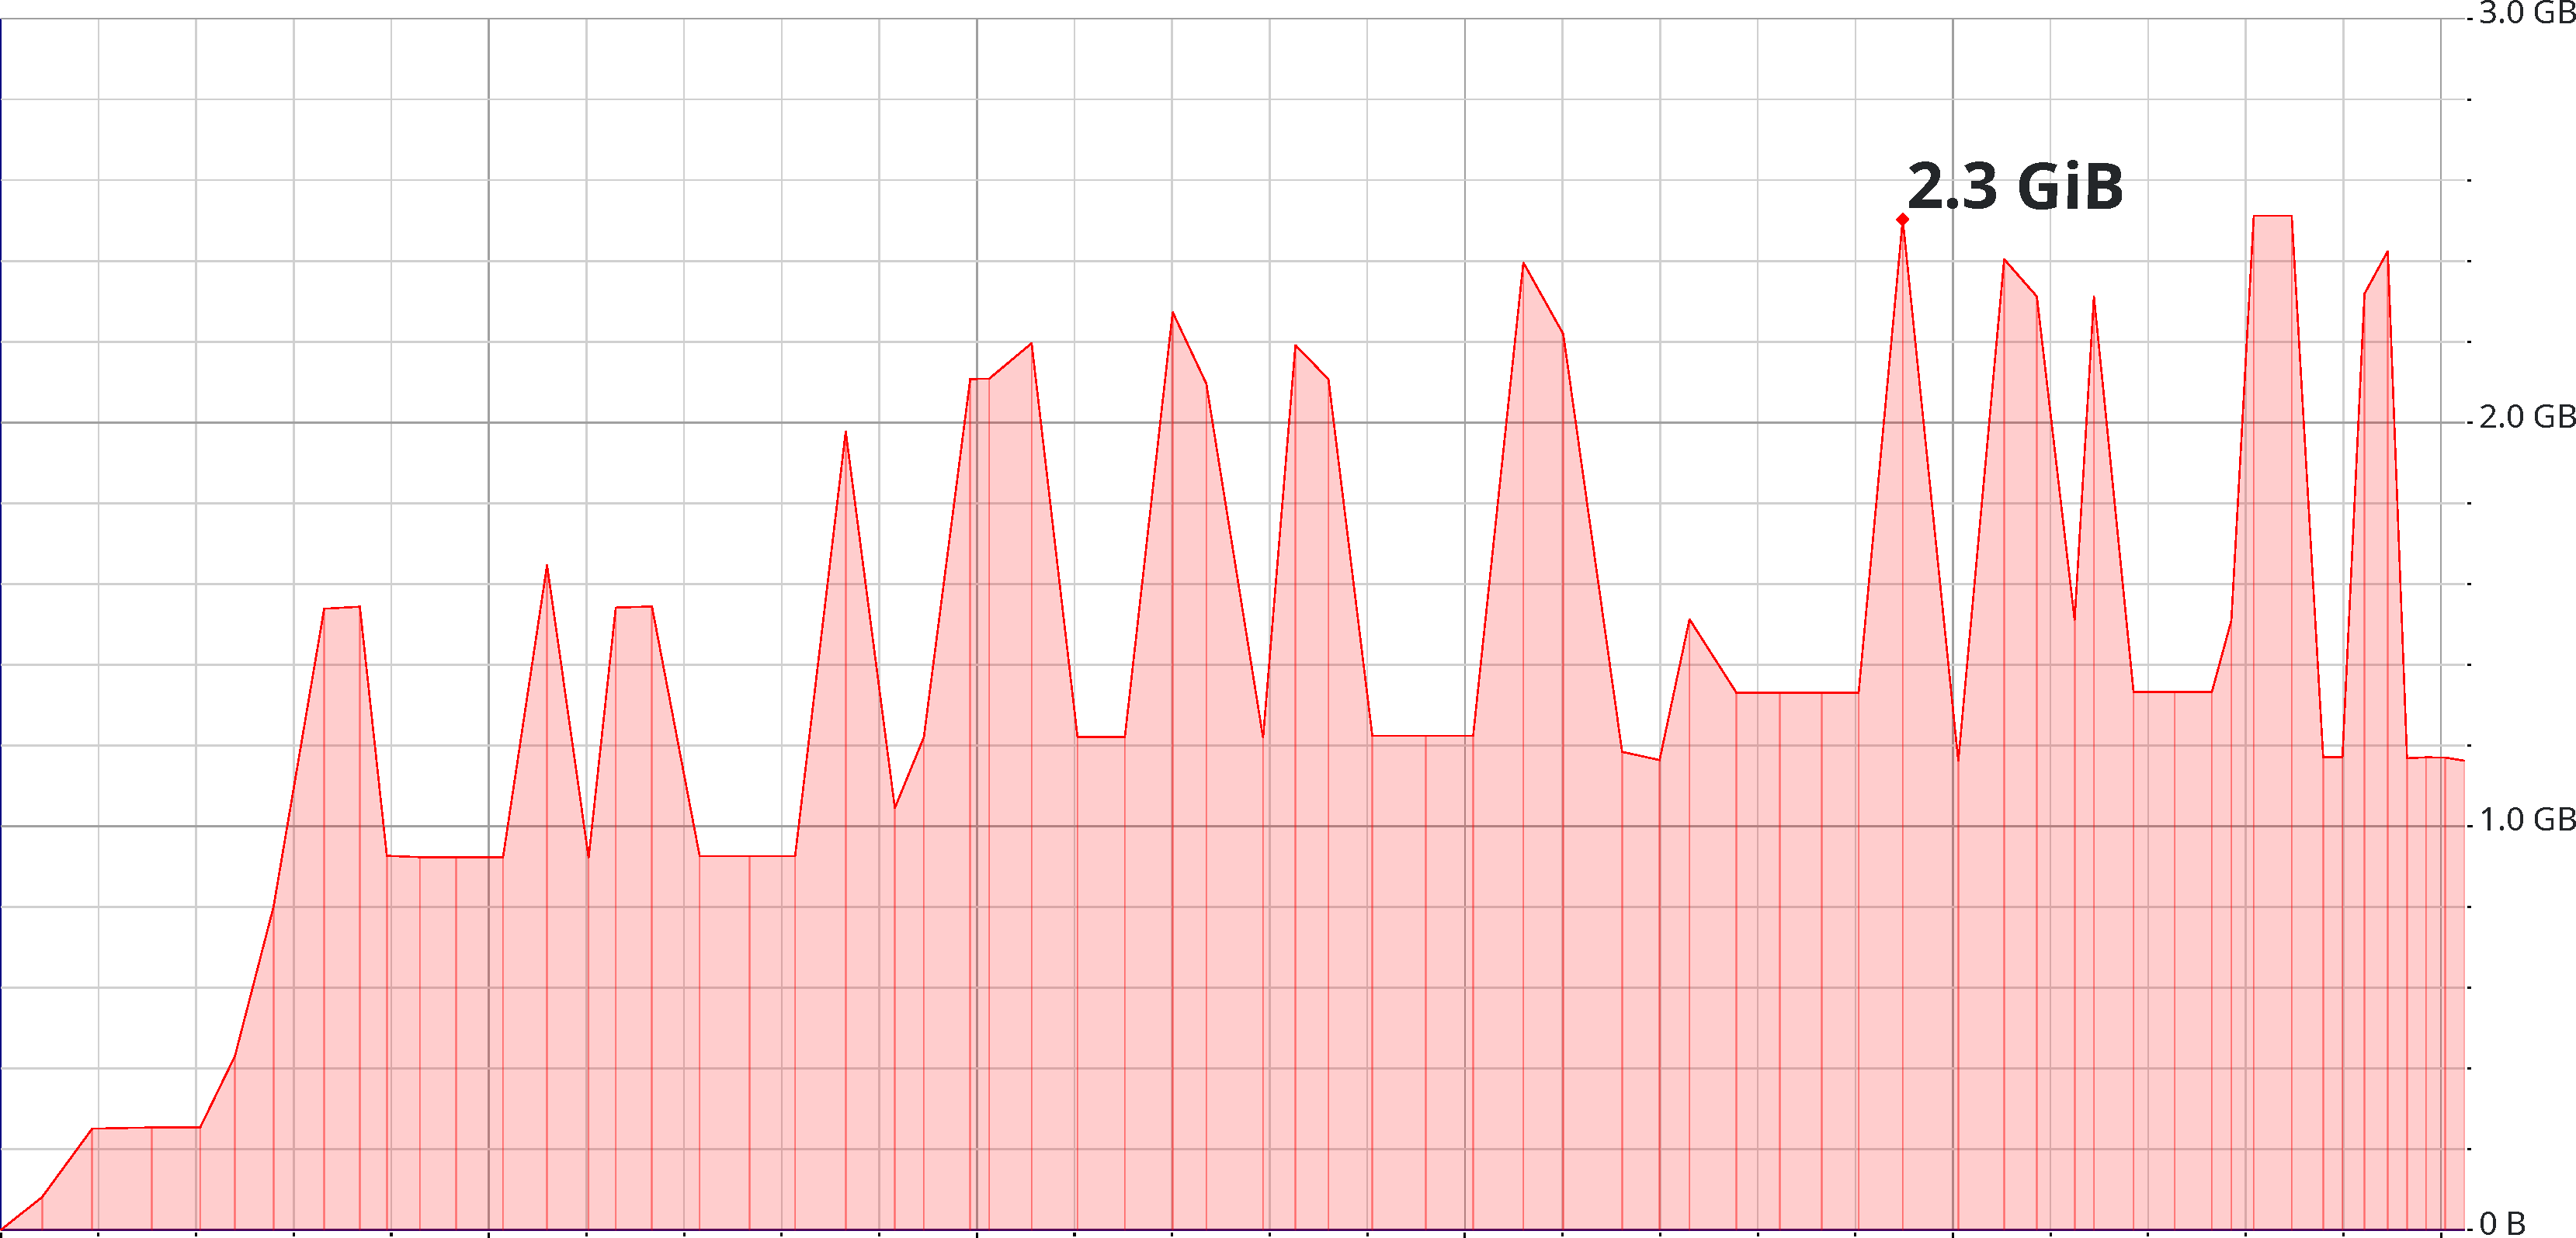
\includegraphics[width=\textwidth]{pictures/mem_prof_patched.pdf}
        \caption{Оптимизированная реализация}
      \end{figure}
      \end{minipage}
  \end{tabular}
  
\end{frame}


\begin{frame}
  \transwipe[direction=90]
  \frametitle{Сравниваемые реализации}
  
  \begin{itemize}
    \item Реализации матричного алгоритма из CFPQ\_PyAlgo для CPU (\textbf{MC}) и GPU (\textbf{MG})
    \item Реализация тензорного алгоритма из CFPQ\_PyAlgo для CPU (\textbf{KC}) и GPU (\textbf{KG}), инкрементальная версия тензорного алгоритма для CPU (\textbf{DKC})
    \item Реализация адаптированного для Points-to анализа, учитывающего поля, тензорного алгоритма (\textbf{OTKC}) и его инкрементальная версия (\textbf{OTDKC});
    \item \textbf{GLL}\footnote{\url{https://github.com/FormalLanguageConstrainedPathQuerying/GLL4Graph}} (запускалась вариация с хранением графа в оперативной памяти)
    \item \textbf{Graspan}\footnote{\url{https://github.com/Graspan/Graspan-C}} (запускался только для анализа псевдонимов, так как эта реализация не поддерживает грамматики с большим количеством нетерминалов)
    \item \textbf{Gigascale}\footnote{\url{https://bitbucket.org/jensdietrich/gigascale-pointsto-oopsla2015}} (запускался только для Points-to анализа, учитывающего поля, так как эта реализация заточена под конкретную грамматику)
  \end{itemize}

\end{frame}


\begin{frame}
  \transwipe[direction=90]
  \frametitle{Время работы: Анализ псевдонимов}

  \begin{center}
      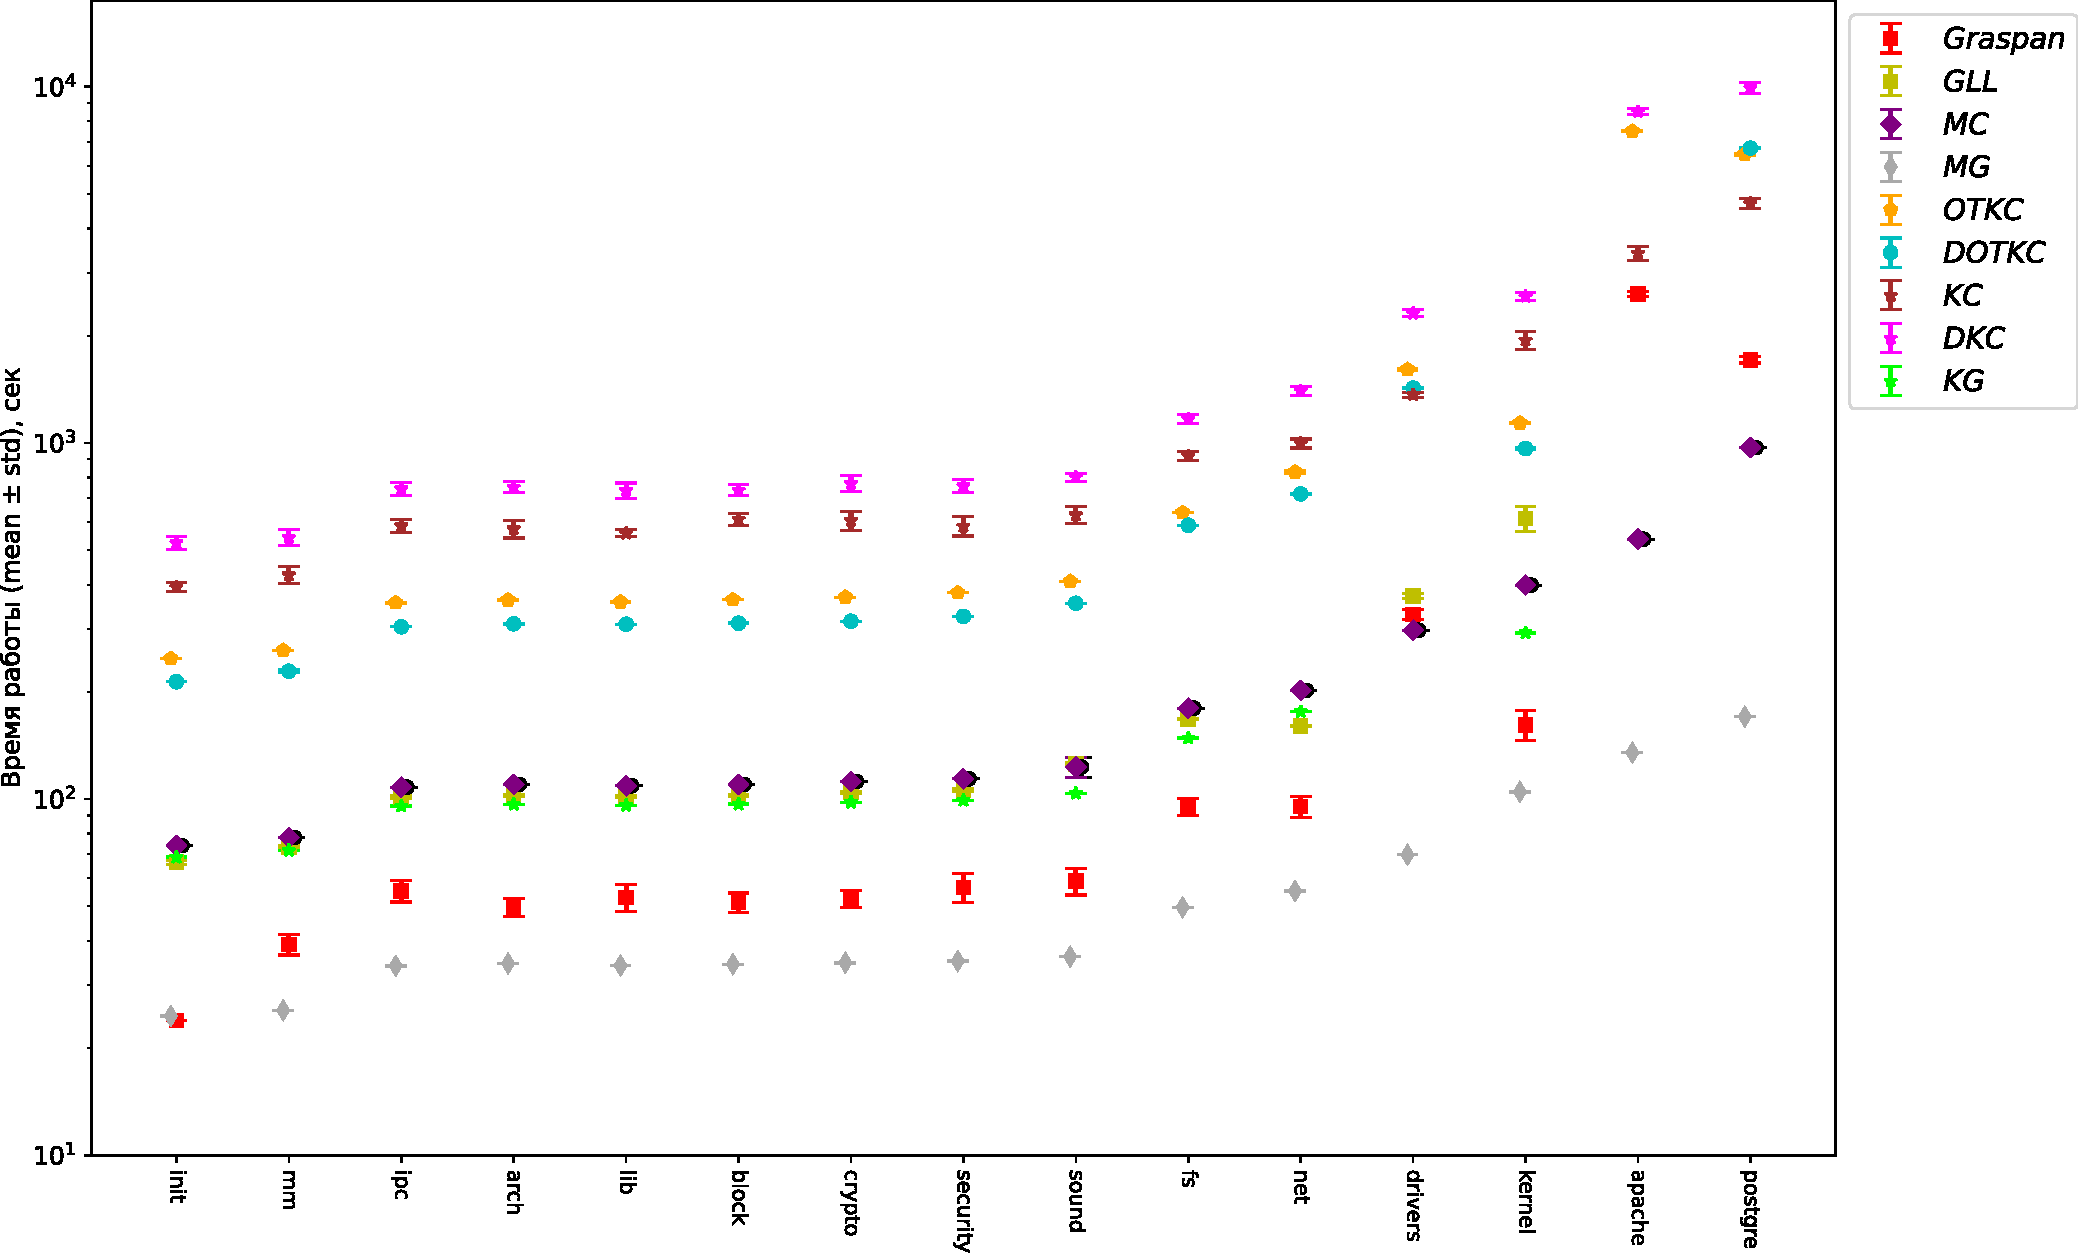
\includegraphics[height=.85\textheight]{pictures/ma_time.pdf}
  \end{center}

\end{frame}

\begin{frame}
  \transwipe[direction=90]
  \frametitle{Время работы: Points-to анализ, учитывающий поля}
  
  \begin{center}
      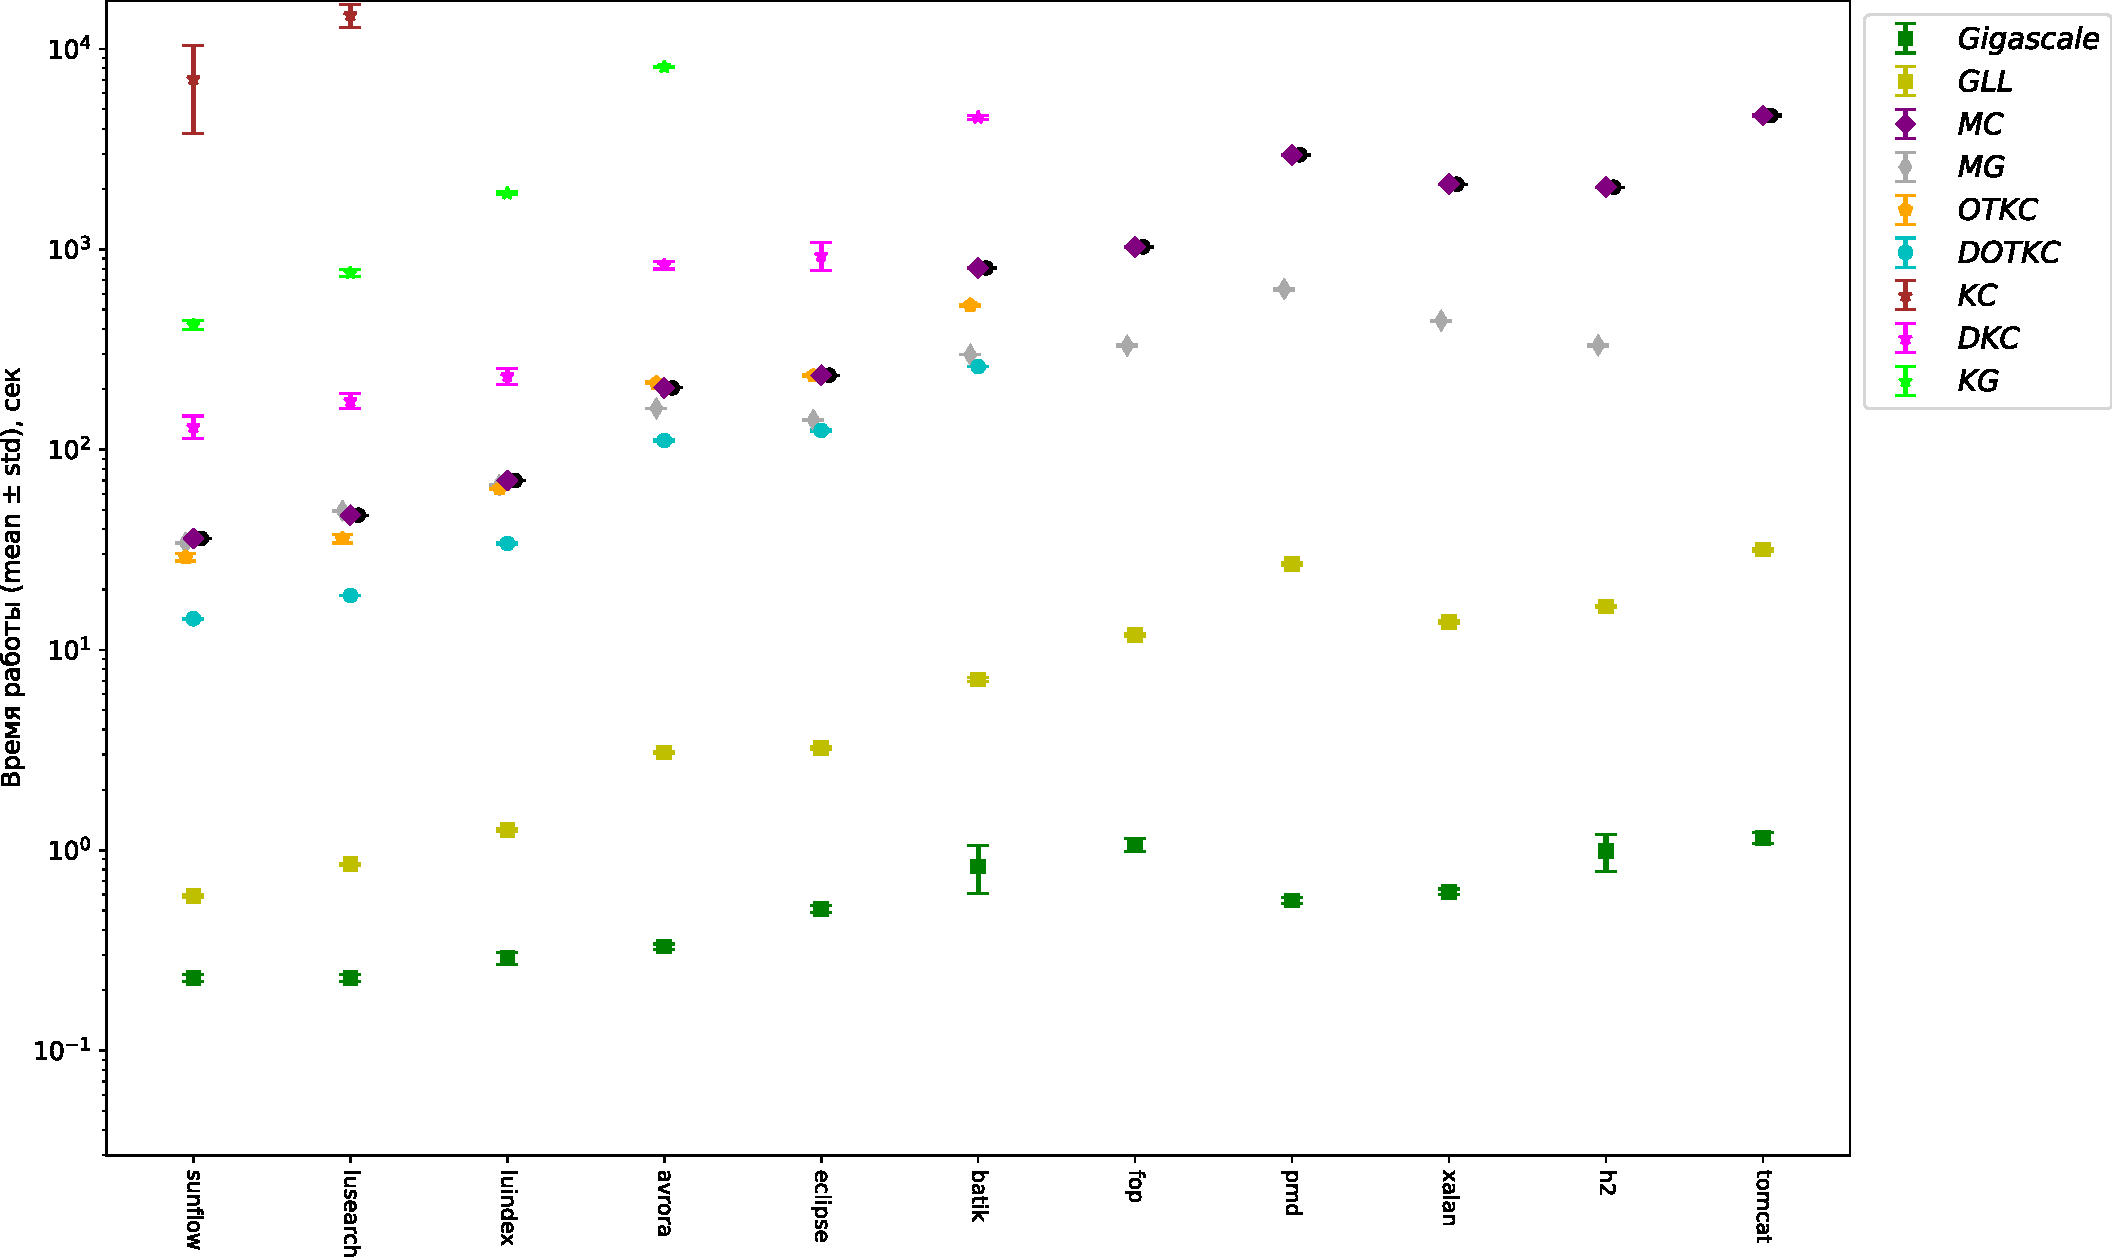
\includegraphics[height=.85\textheight]{pictures/java_time.pdf}
  \end{center}

\end{frame}


\begin{frame}
  \transwipe[direction=90]
  \frametitle{Результаты}
  \begin{itemize}
    \item Для Points-to анализа, учитывающего поля, была предложена модификация тензорного алгоритма. Данная модификация была реализована в рамках библиотеки CFPQ\_PyAlgo
    \item Оптимизирована реализация матричного алгоритма из библиотеки CFPQ\_PyAlgo, эффективность оптимизации экспериментально проверена
    \item Проведены замеры производительности реализаций алгоритмов КС-достижимости
  \end{itemize}

\end{frame}


\appendix


\begin{frame}[fragile]\
    \frametitle{Ответы на вопросы и замечания}
    
    \begin{itemize}
        \item Корректность
        \begin{itemize}
            \item Анализ псевдонимов
            \begin{itemize}
                \item Program analysis via graph reachability\footnote{\url{https://dl.acm.org/doi/10.5555/271338.271343}} (Thomas Reps)
                \item Demand-Driven Alias Analysis for C\footnote{\url{https://dl.acm.org/doi/10.1145/1328897.1328464}} (Xin Zheng and Radu Rugina)
            \end{itemize}
            \item Points-to анализ, учитывающий поля
            \begin{itemize}
                \item Refinement-based context-sensitive points-to analysis for Java\footnote{\url{https://dl.acm.org/doi/10.1145/1133981.1134027}} (M. Sridharan and R. Bodik)
            \end{itemize}
        \end{itemize}
        \item Для графа $\mathcal{G}=\langle V,E,l \rangle$ и грамматики $G=\langle \Sigma, N, P, S \rangle$ вычислительная сложность
        \begin{itemize}
            \item Матричный алгоритм --- $O(|N||P||V|^5)$
            \item Тензорный алгоритм --- $O(|P|^3|V|^3 / \log{(|P||V|)})$
        \end{itemize}
    \end{itemize}
\end{frame}

\end{document}
